\documentclass[article,colorback,accentcolor=tud4c]{tudreport}
\usepackage{ngerman}

\usepackage[stable]{footmisc} 
\usepackage[ngerman]{hyperref}
\usepackage[utf8]{inputenc}
\usepackage{longtable}
\usepackage{multirow}
\usepackage{booktabs}
\usepackage{pst-all}
\usepackage{amsmath}
\usepackage{subfigure}


% Makros
\newcommand{\before}[1]{\textit{ before(#1) }}
\newcommand{\after}[1]{\textit{after(#1)}}
\newcommand{\aktiv}[1]{\textit{active(#1)}}
\newcommand{\Interval}[1]{\textbf{interval#1}}
\newcommand{\comp}[1]{\textit{comp(#1)}}
\newcommand{\val}[1]{\textit{value(#1)}}

\hypersetup{%
  pdftitle={TUD Corporate-Design f"ur {\LaTeX}}, pdfauthor={C. v. Loewenich und
  J. Werner}, pdfsubject={Beispieltext}, pdfview=FitH, pdfstartview=FitV }

\setcounter{seclinedepth}{1}

  \newif\ifTUDmargin\TUDmarginfalse \ifTUDmargin\makeatletter
    \TUD@setmarginpar{2}
  \makeatother\fi

\newlength{\longtablewidth}
\setlength{\longtablewidth}{0.7\linewidth}
\addtolength{\longtablewidth}{-\marginparsep}
\addtolength{\longtablewidth}{-\marginparwidth}

\title{IntervalEvents in EScala: Design}
\subtitle{Michael Kutschke und Frank Englert}

\begin{document}

\maketitle

\tableofcontents

\section{Grundlegende Definitionen}
\label{definitions}
Sei \before{\Interval} : Event das Ereignis, das den Beginn des Intervalls int angibt
und \after{\Interval} : Event jenes, welches das Ende des Intervalls angibt.
Hierbei sind folgende Event-Sequenzen zulässig:
\begin{itemize}
\item einmal \before{\_} zu Beginn und einmal \after{\_} am Ende
\item mehrfaches \before{\_} und ein \after{\_} am Ende 
\item verschachtelte, paarweise passende \before{\_} und \after{\_} Ereignisse
%\item beliebige \before{\_} und \after{\_} Events innerhalb des Intervals
\end{itemize}
Ausserdem gebe \aktiv\Interval{} : boolean an, ob das Intervall aktiv ist.
In der jetzigen Fassung bedeutet dies einfach, ob man sich zeitlich innerhalb des
Intervalls befindet. 
Der Wert des Active-Flags hat dabei die in Abb.
\ref{active_bit_behaviour} gezeigte Semantik. Zum Zeitpunkt des
Before-Events ist \aktiv\Interval{} noch nicht gesetzt. Dies ist keine
Einschr"ankung, wie im weiteren gezeigt werden wird. 

\begin{figure}[h]
 \centering 
\psset{unit=1cm} 
\begin{pspicture}(0,0)(10,2)
\psgrid[subgriddiv=1,griddots=10,gridlabels=7pt,](0,0)(10,2)
%{
%	\pspolygon[fillcolor=greenyellow,fillstyle=solid,linestyle=none](0,0)(0,1)(1,1)(1,0)

	\rput(1.2,0.7){\psframebox*[framearc=.3]{B}}
	\rput(9.2,0.7){\psframebox*[framearc=.3]{A}}
	\rput(0.2,1.05){\psframebox*[framearc=.3]{Aktiv}} 
	\psline[linewidth=1pt]{]-]}(1,1)(9,1)
%}
\end{pspicture}
\caption{Wert des Aktiv-Bits}
\label{active_bit_behaviour}
\end{figure}


F"ur alle Intervalle muss gelten, dass active nur beim \before{\_} oder
\after{\_} Event umgeschaltet wird, wobei \aktiv{\_} nur von einem \before{\_}
Event gesetzt und von einem \after{\_} Event zur"uckgesetzt werden kann.
Ausserdem sollten ausserhalb des Intervalls keine isolierten Events auftreten.

\section{Operatoren}
Im folgenden werden die auf Intervall-Events verfügbaren Operatoren definiert:

\subsection{Komplement \comp\Interval : Intervall}
\begin{itemize}
\item \before{\comp{\Interval}} <=> \after{\Interval}
\item \after{\comp{\Interval}} <=> \before{\Interval} 
\item \aktiv{\comp{\Interval}} <=> ! \aktiv{\Interval}
\end{itemize}
Bei der Implementierung wird ein neues Intervall-Event erzeugt, bei dem das 
Before-Event mit dem After-Event getauscht ist. Das Komplement bietet keinen
Zugriff auf den Value des Intervall-Events.

\subsection{Vereinigung \Interval{1} || \Interval{2} : Intervall}
Die Semantik der ||-Vereinigung ist die Vereinigung der Zeitpunkte von
\Interval{1} und \Interval{2}.
\begin{itemize}
\item \before{\Interval{1} || \Interval{2}}  <=> (\before{\Interval{1}} ||
\before{\Interval{2}}) \&\& !
\aktiv{\Interval{1} || \Interval{2}}
%(((after && (_ => !ie.active)) || 
% (ie.after && (_ => !active)) || 
% (after and ie.after))) \ (before || ie.before), active || 
% ie.active, _value)
\item \after{\Interval{1} || \Interval{2}} <=> \after{\Interval{1}} \&\&
!\aktiv{\Interval{2}} || \after{\Interval{2}} \&\& !\aktiv{\Interval{1}} ||
\after{\Interval{1}} \&\& \after{\Interval{2}}except(\before{\Interval{1}}||\before{\Interval{2}})

\end{itemize}

\subsection{Schnitt \Interval{1} \&\& \Interval{2} : Intervall}
\begin{itemize}
\item \before{\Interval{1} \&\& \Interval{2}} <=> (((\before{\Interval{1}} \&\& \aktiv{\Interval{2}}) ||
(\before{\Interval{2}} \&\& \aktiv{\Interval{1}}) || (\before{\Interval{1}} \&\& \before{\Interval{2}}))
\textbackslash (\after{\Interval{1}} || \after{\Interval{2}})) \&\& ! \aktiv{\Interval{1} \&\& \Interval{2}}
\item \after{\Interval{1} \&\& \Interval{2}} <=> \before{\comp{\Interval{1}}} ||
\before{\comp{\Interval{2}}}
\item \aktiv{\Interval{1} \&\& \Interval{2}} <=> \aktiv{\Interval{1}} \&\& \aktiv{\Interval{2}}
\end{itemize}

\subsection{Differenz \Interval{1} \textbackslash\ \Interval{2} : Interval}
Alle Zeitpunkte, die in \Interval{1} liegen, nicht aber in \Interval{2}:
\begin{itemize}
  \item  \Interval{1} \textbackslash\ \Interval{2} <=> \Interval{1} \&\&
  comp(\Interval{2})
\end{itemize}


\subsection{within(\Interval{},e) : Event}
within(\Interval{},e) <=> (e \&\& \aktiv{\Interval}) || (e \&\& \before{\Interval})

\subsection{!within(\Interval{},e) : Event}
!within(\Interval{},e) <=> (e \&\& ! \aktiv{\Interval}) \textbackslash\ \before{\Interval}

\subsection{ StrictlyWithin(\Interval{},e) : Event}
StrictlyWithin(\Interval{},e) <=> (e \&\& \aktiv{\Interval}) \textbackslash\ \after{\Interval}

\subsection{ !strictlyWithin(\Interval{},e) : Event }
!strictlyWithin(\Interval{},e) <=> (e \&\& ! \aktiv{\Interval}) || (e \&\& \after{\Interval})


\subsection{weitere Anmerkungen}
Der Umstand, dass sich int und \comp{\Interval{}} zwei Zeitpunkte teilen, mag
unintuitiv erscheinen, allerdings  bietet dies nicht nur Nachteile. So ist int
|| \comp{\Interval{}} wie  erwartet immer aktiv, beginnt und endet niemals. int
\&\& \comp{\Interval{}} ist niemals aktiv  und l"ost auch niemals before oder
after Ereignisse aus.

  \section{An Events gebundene Werte}
Es ist m"oglich, beliebige Werte an Events zu binden. Diese M"oglichkeit
existiert auch f"ur Intervall-Events. Wann im Intervall welche Werte
gelten, h"angt von der Art des Intervalls ab. 

Auf den aktellen Wert des Intervalls wird "uber \val(\Interval{})
zugegriffen. 

Nachfolgend wird das Standartverhalten der Intervall-Operatoren dargestellt.
Allerdings kann das Verhalten der Operatoren bei Bedarf abge"andert werden. Dann
muss beim Intervall-Event-Knoten eine Benutzerdefinierte Merge-Funktion
angegeben werden, die Values der Events aggregiert.

\subsection{Intervall zwischen dem Event B und dem Event A)}
F"ur between-Intervalle wie in Abbildung \ref{interval-between_b_a} gilt der Wert des
Before-Events bis zum End-Event. Dannach hat das Intervall den Wert null. Der
Wert des After-Events wird allerdings nicht im Komplement gespeichert. Beim
Intervall\ref{interval-between_b_a} gilt also:
\[
val(t) = \begin{cases}
null & t < 1 \\
B.val & t >= 1 \; and \; t < 9 \\
null & t >= 9
\end{cases}
\]

\begin{figure}[h]
 \centering 
\psset{unit=1cm}
\begin{pspicture}(0,0)(10,2)
\psgrid[subgriddiv=1,griddots=10,gridlabels=7pt](0,0)(10,1)
%{
%	\pspolygon[fillcolor=greenyellow,fillstyle=solid,linestyle=none](0,0)(0,1)(1,1)(1,0)

	\rput(1.2,0.7){\psframebox*[framearc=.3]{B}}
	\rput(9.2,0.7){\psframebox*[framearc=.3]{A}}
	\psline[linewidth=1pt]{[-]}(1,0.5)(9,0.5)
%}
\end{pspicture}
\caption{Intervall-Event between(B,A)}
\label{interval-between_b_a}
\end{figure}



Wenn die \before{\_}-Events mehrfach auftreten, hat das
between-Intervall den Wert des ersten \before{\_}-Events. Ein Beispiel hierf"ur ist in Abbildung
\ref{interval-between_b_a-multiple} zu sehen. F"ur
Interval\ref{interval-between_b_a-multiple} gilt \[ val(t) =
\begin{cases}
null & t < 1\\
B.val &  t >= 1 \; and \; t < 7\\
null  & t >= 7
\end{cases}
\]

\begin{figure}[h]
 \centering 
\psset{unit=1cm}
\begin{pspicture}(0,0)(10,2)
\psgrid[subgriddiv=1,griddots=10,gridlabels=7pt](0,0)(10,1)
%{
	\rput(1.2,0.75){\psframebox*[framearc=.3]{B}}
	\rput(7.2,0.75){\psframebox*[framearc=.3]{A}}
	\psline[linewidth=1pt]{[-]}(1,0.5)(7,0.5)
	
	\rput(3.2,0.75){\psframebox*[framearc=.3]{B'}}
	\rput(9.2,0.75){\psframebox*[framearc=.3]{A'}}
	\psline[linewidth=1pt,linestyle=dotted]{[-]}(3,0.5)(9,0.5)
%}
\end{pspicture}
\caption{Intervall-Event between(B,A) mit mehrfach auftretenden Before- und
After-Events}
\label{interval-between_b_a-multiple}
\end{figure}
 
 
\subsection{Vereinigung von Intervallen}
F"ur die Vereinigung von Intervallen ist es sinnvoll, den Wert des letzen
\before{\_}-Events zu speichern. Damit hat man immer Zugriff auf den Wert des
letzten Events, der die Bedingung erf"ullt hat. 

\begin{figure}[h]
 \centering 
\psset{unit=1cm}
\begin{pspicture}(0,0)(10,4)
\psgrid[subgriddiv=1,griddots=10,gridlabels=7pt](0,0)(10,3)
%{
	\rput(1.2,2.75){\psframebox*[framearc=.3]{B}}
	\rput(7.2,2.75){\psframebox*[framearc=.3]{A}}
	\psline[linewidth=1pt]{[-]}(1,2.5)(7,2.5)
	
	\rput(3.2,1.75){\psframebox*[framearc=.3]{B'}}
	\rput(9.2,1.75){\psframebox*[framearc=.3]{A'}}
	\psline[linewidth=1pt]{[-]}(3,1.5)(9,1.5)
	
	\rput(1.2,0.75){\psframebox*[framearc=.3]{B}}
	\rput(9.2,0.75){\psframebox*[framearc=.3]{A'}}
	\psline[linewidth=1pt]{[-]}(1,0.5)(9,0.5)
%}
\end{pspicture}
\caption{Vereinigung zweier Intervall-Events: between(B,A) || between(B',A')}
\label{interval-or}
\end{figure}
  
F"ur das in Abb\ref{interval-or} zu sehende Interval\ref{interval-or}
between(A,B) || between(A',B') gilt also die folgende Belegung des Wertes:
\[
val(t) = \begin{cases}
null & t < 1 \\
B.val & t >=1 \; and t < 3 \\
B'.val & t >=3 \; and t < 9 \\
null & t > 9 \\
\end{cases}
\]
  
  \subsection{Schnittmenge zwischen Intervallen}
Bei der Schnittmenge zwischen zwei Intervall-Events werden die Event-Werte der
beiden aktiven Interval-Events zu einem Tupel zusammengefasst. 

\begin{figure}[h]
 \centering 
\psset{unit=1cm}
\begin{pspicture}(0,0)(10,4)
\psgrid[subgriddiv=1,griddots=10,gridlabels=7pt](0,0)(10,3)
%{
	\rput(1.2,2.75){\psframebox*[framearc=.3]{B}}
	\rput(7.2,2.75){\psframebox*[framearc=.3]{A}}
	\psline[linewidth=1pt]{[-]}(1,2.5)(7,2.5)
	
	\rput(3.2,1.75){\psframebox*[framearc=.3]{B'}}
	\rput(9.2,1.75){\psframebox*[framearc=.3]{A'}}
	\psline[linewidth=1pt]{[-]}(3,1.5)(9,1.5)
	
	\rput(3.2,0.75){\psframebox*[framearc=.3]{(B,B')}}
	\rput(7.2,0.75){\psframebox*[framearc=.3]{(A', A)}}
	\psline[linewidth=1pt]{[-]}(3,0.5)(7,0.5)
%}
\end{pspicture}
\caption{Schnittmenge zweier Intervall-Events: between(B,A) and
between(B',A')}
\label{interval-and}
\end{figure}

Wie in Abb. \ref{interval-and} zu sehen, ergibt sich das folgende Zeitliche
Verhalten f"ur den Wert von Interval\ref{interval-and} \[
val(t)=\begin{cases}
null & t < 3 \\
(B,B') & t >=3 \; and t <= 7 \\
null & t > 7
\end{cases}
\]

\subsection{Differenz zweier Intervall-Events}
Bei der Differenz zwischen zwei Intervall-Events ist der Wert des Intervalls
gleich dem Wert des letzten Before-Events vor oder nach dem Schnitt.

\begin{figure}[h]
 \centering 
\psset{unit=1cm}
\begin{pspicture}(0,0)(10,4)
\psgrid[subgriddiv=1,griddots=10,gridlabels=7pt](0,0)(10,3)
%{
	\rput(1.2,2.75){\psframebox*[framearc=.3]{B}}
	\rput(4.2,2.75){\psframebox*[framearc=.3]{A}}
	\psline[linewidth=1pt]{[-]}(1,2.5)(4,2.5)
	
	\rput(6.2,2.75){\psframebox*[framearc=.3]{B''}}
	\rput(9.2,2.75){\psframebox*[framearc=.3]{A''}}
	\psline[linewidth=1pt]{[-]}(6,2.5)(9,2.5)
	
	\rput(3.2,1.75){\psframebox*[framearc=.3]{B'}}
	\rput(5.2,1.75){\psframebox*[framearc=.3]{A'}}
	\psline[linewidth=1pt]{[-]}(3,1.5)(5,1.5)
	
	\rput(1.2,0.75){\psframebox*[framearc=.3]{B}}
	\rput(3.2,0.75){\psframebox*[framearc=.3]{B'}}
	\psline[linewidth=1pt]{[-]}(1,0.5)(3,0.5)
	
	\rput(6.2,0.75){\psframebox*[framearc=.3]{B''}}
	\rput(9.2,0.75){\psframebox*[framearc=.3]{A''}}
	\psline[linewidth=1pt]{[-]}(6,0.5)(9,0.5)
%}
\end{pspicture}
\caption{between(B,A) except between(B',A')}
\label{interval-diff}
\end{figure}

F"ur Interval\ref{interval-diff} = between(B,A) except between(B', A') ergibt
sich also folgende Belegung:
\[
val(t)=\begin{cases}
null & t < 1 \\
B & t \in [1,3] \\
null & t \in [3,6] \\
B'' & t\in[6,9]\\
null & t >9
\end{cases}
\]

\section{Implementierung}

Die Implementierung der Interval-Events hat das gleiche Schema wie die
Implementierung der Events. Es handelt sich bei Intevall-Events um eine
spezielle Form von Event-Nodes die aus einem Start- und einem Stop-Event
bestehen.

Wie bei jedem Event-Node aus dem scala.events-Package durchl"auft ein
Intervall-Event einen Lebenszyklus bestehend aus dem Setup des Event-Graphen,
der Registrierung von Reactions, dem Deploy, der Unregistrierung von Reactions
und dem Undeploy von Event-Nodes. Dieser Lebenszyklus ist auch in
Abb. \ref{event_node_lifecycle} zu sehen.

%\usepackage{graphics} is needed for \includegraphics
\begin{figure}[htp]
\begin{center}
  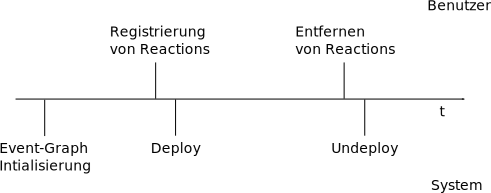
\includegraphics[width=0.7\textwidth]{graphics/EventNode-Lifecycle}
  \caption{Lifecycle eines EventNodes}
  \label{event_node_lifecycle}
\end{center}
\end{figure}


Es gibt, wie in Abb.\ref{interval_events_structure} zwei Klassen von
Intervall-Event-Nodes: BetweenEvents und ExecutionEvents. BetweenEvents sind vom
Auftreten des StartEvents bis zum Auftreten des ersten End-Events aktiv, wenn
eine Reaction registiert wurde. Das Execution-Event dient dazu, die Ausf"uhrung
einer Funktion zu protokollieren. Wenn das Execution-Event eine Funktion
"uberwachen soll, dann instrumentiert der Compiler die Funktion so, dass ein
Before-Event beim Betreten der Funktion und ein After-Event beim Verlassen der
Funktion ausgel"ost wird.

%\usepackage{graphics} is needed for \includegraphics
\begin{figure}[htp]
\begin{center}
  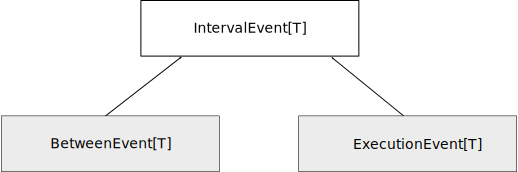
\includegraphics[width=0.5\textwidth]{graphics/interval_event_structure}
  \caption{Arten von Intervall-Events}
  \label{interval_events_structure}
\end{center}
\end{figure}

\subsection{Die Klasse IntervalEvent}
Die Klasse IntervalEvent stellt folgende Methoden zur Verfügung:

\begin{description}
\item{\bf before: } Das zum Interval zugehörige before-Ereignis wie oben definiert
\item{\bf after: } das after-Ereignis, wie oben definiert
\item{\bf value: } der Wert des Intervals, wie oben definiert. Zusätzlich wird via pull eine punktgenaue Abfrage ermöglicht,
Unterklassen sollten jedoch getValue stattdessen verwenden und Spezialfälle (Endpunkte des Intervals) gesondert behandeln
\item{\bf isActive: } den Wert des Active-Bits, wie oben definiert. Zusätzlich wird via pull der Anfangspunkt des Intervals eingeschlossen. Unterklassen sollten stattdessen active verwenden und den Spezialfall gesondert behandeln.
\item{\bf complement,\&\&,||,\textbackslash: } wie oben definiert
\item{\bf map(V => T):IntervalEvent[T] : } transformiert den Wert des Intervals
\item{\bf \&\&(\Interval{2},(V => Boolean)): } filtert Intervalle nach Werten
\end{description}

Zusätzlich stellt das Package scala.events die Methode \textit{Lazy(\Interval{})} zur Verfügung, die für die Deklaration von rekursiv oder zyklisch voneinander abhängigen Intervallen gebraucht werden kann. \textit{from} und \textit{to} erlauben die Definition von Intervallen, die nur einen Start- bzw. Endpunkt besitzen.

\subsection{Der Aufbau des Event-Graphen}
Mithilfe von Event-Nodes k"onnen mehrere Events zu komplexeren Events
zusammengefasst werden. So ist es beispielsweise m"oglich, alle Events einer
Filter-Bedingung zu unterziehen. Das resultierende Event wird nur dann
ausgel"ost, wenn ein zu filterndes Event auftritt dessen Filterbedingung zu
wahr auswertet. 

Der aus mehreren Event-Knoten bestehende Abhänigkeitsgraph soll nachfolgend als
Event-Graph bezeichnet werden. Ein Event-Graph besteht aus mindestens einem
Event-Node. Mehrere Event-Nodes können mit gerichteten Kanten verbunden sein. 
Es gibt zwei Arten von Kanten im Event-Graphen. Unbeschriftete Kanten zeigen 
die ``Flussrichtung'' von Events an. Kanten die mit pull() beschriftet sind, 
zeigen die zu prüfenden Abhängigkeiten bei einer Pull-Operation an. 
Except-Event-Knoten haben die Beschriftung ``$\backslash$''.

Wenn Intervall-Events im Eventgraph verwendet werden sollen, müssen die zum
Intervall gehörigen before- oder after-Events in den Eventgraph eingefügt
werden. Eine Liste der m"oglichen Filterfunktionen und die dazugeh"origen 
Definitionen findet sich im Kapitel \ref{definitions}.

\subsection{Auswertung des Eventgraphen}

Bei der Auswertung eines Event-Graphen gibt es zwei mögliche Vorgehensweisen.
Zum einen kann man Events sammeln, die bei einem Knoten des Event-Graphen
ankommen und dann weiterleiten, wenn gewisse Bedingungen erfüllt sind. Hierbei handelt es sich um
eine Push-basierte Implementierungen. Es werden n"amlich nur "Anderungen gepusht.

Beim Zweiten Ansatz werden keine Änderungen weitergeleitet. Stattdessen wird
der Event-Graph traversiert um herauszufinden, ob Änderungen passiert sind. Dieser
Ansatz wird nachfolgend als Pull-basiert bezeichnet.

Bei gleichem Resultat haben beide Implementierungen verschiedene Vor- und
Nachteile. Nachteilig beim Push-basierten Ansatz ist die relativ hohe Komplexität
der Implementierung wenn Knoten im Event-Graph einen Zustand aufweisen.
Dann ist es schwierig, ein deterministisches Verhalten sicherzustellen. Beim
Pull-basierten Ansatz stellt sich stattdessen die Frage, wie man den richtigen
Zeitpunkt f"ur einen Pull ermitteln kann. 

Die Implementierung im scala.events-Modul verwendet einen hybriden Ansatz um den
Event-Graphen auszuwerten. Die meisten Event-Knoten wurden Push-basiert
implementiert. Eine Ausnahme stellt der Except-Knoten dar. Mit einem solchen
Event-Knoten k"onnen verschiedene Events ausgeschlossen werden. Der Except-Zweig
des Event-Knotens wurde pull-basiert implementiert.

Betrachten wir nachfolgend zwei Beispiele um diese Vorgehensweise zu begr"unden:
\begin{eqnarray}
val \; e & = e1 \setminus (e2 || e3)\\
val \; e & = e1 \setminus (e1 || e3)
\end{eqnarray}

Der Event-Graph des Push-basierten Ansatzes ist in
Abb.\ref{push_based_event_graph} zu sehen. Wenn das Event e1 ausgelöst wird,
startet zunächst das Sammeln von Reactions im Knoten e1 und folgt den im
Diagramm eingezeichneten Kanten. 
 
Der Except-Event-Knoten speichert intern ob bereits ein Sammelvorgang über den
Except-Zweig durchgeführt wurde. Ist dies nicht der Fall, dann wird das Sammeln
in e forgesetzt und die Reaction auf das Event e wird gesammelt. 

Wenn allerdings schon eine Sammlung über den Except-Zweig erfolgte, dann
verhindert der Except-Knoten das Sammeln der Reactions von e.

Der in Abb.\ref{pull_based_event_graph} beschriebene Ansatz funktioniert
prinzipiell genauso. Allerdings wird im Except-Event-Node explizit der Pull-Vorgang ausgelöst um zu
prüfen, ob die Except-Bedingung gilt oder nicht. Der Except-Knoten speichert
dann keinen internen Zustand mehr.

Betrachten wir nun das Beispiel 2. Das Beispiel 2 ist praktisch von keiner
Bedeutung. Allerdings zeigt es gut die Probleme einer Push-basierten
Implementierung auf. 

Wenn der Event e1 ausgelöst wird, kann das Sammeln von Reactions nun mit zwei
Knoten starten wie man im Event-Graphen in Abb.
\ref{failing_push_based_event_graph} sehen kann. Möglicherweise werden die
Reactions vom Except-Knoten über den Or-Knoten zuerst gesammelt. Dann schaltet 
der Except-Knoten seinen internen Zustand um. Wenn anschließend die Sammlung
über  die zweite Kante von e1 erfolgt, hat sich der Zustand von Except bereits 
geändert, sodass keine Reaktionen von e gesammelt werden.

Wenn allerdings zunächst der Except-Knoten besucht wird, hat dieser seinen
internen Zustand noch nicht umgeschaltet. Dann werden die Reactions von e
gesammelt. Erst wenn später der Except-Knoten über den Or-Knoten besucht wird,
schaltet der Except-Knoten seinen Zustand um. Allerdings wurde dann schon die
Reaction von e gesammelt. Daher muss, wenn der Except-Knoten über den
Except-Zweig erreicht wird, die Liste mit Reactions gelöscht werden. Das hier
genannte Beispiel 2 würde dann korrekt arbeiten. Allerdings lassen sich durch
kompliziertere Beispiele Zustände erzeugen, bei dem das korrekte Sammeln von
Events scheitert\footnote{Ein Beispiel hierfür ist ein Event-Graph bei dem sich
über dem Except-Knoten ein And-Knoten befindet}.

Der Pull-basierte Ansatz ist in Abb. \ref{working_pull_based_event_graph} zu
sehen. Hier gibt es in e1 nur einen Weg, die Sammlung der Reactions zu
beginnen\footnote{Natürlich gibt es auch hier wieder zwei Wege von e1 zum
Except-Knoten. Allerdings stellt der Weg über den Or-Knoten eine Sackgasse
dar. Sammler die den Except-Knoten über diesen Weg erreichen, werden ignoriert
und sammeln keine Reactions ein.}. Wenn der Reaction-Sammler nun im
Except-Event-Knoten angelangt, wird eine Pull-Operation auf den Except-Zweig ausgeführt. Dabei  wird
festgestellt, dass der auslösende Event ebenfalls über die Except-Kante beim 
Except-Knoten ankommt. Daher werden keine Reactions von e gesammelt.


 


%\usepackage{graphics} is needed for \includegraphics
\begin{figure}[htp]
\centering
\subfigure[Push basierter Event-Gaph] {
  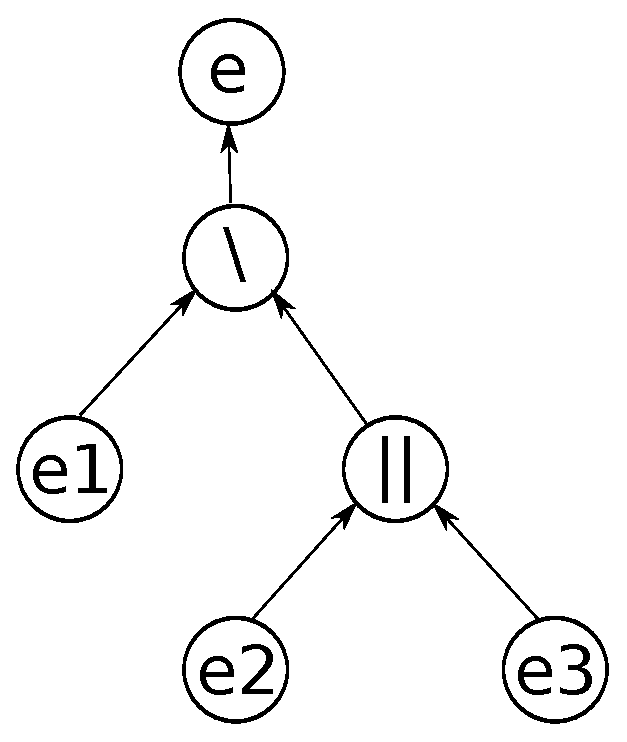
\includegraphics[width=0.3\textwidth]{graphics/event_node_except_push}
  \label{push_based_event_graph}
}
\subfigure[Push/Pull basierter Event-Graph] {
  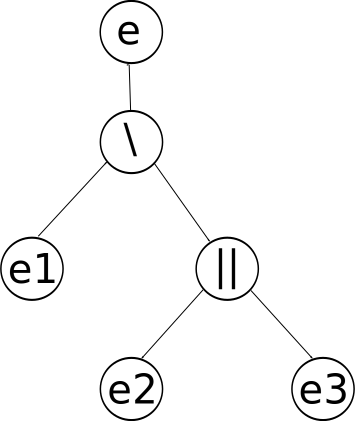
\includegraphics[width=0.3\textwidth]{graphics/event_node_except_pull}
  \label{pull_based_event_graph}
}
\caption{Event-Graphen f"ur das Beispiel 1}
\end{figure}

\begin{figure}[htp]
\centering
\subfigure[Push basierter Event-Gaph] {
  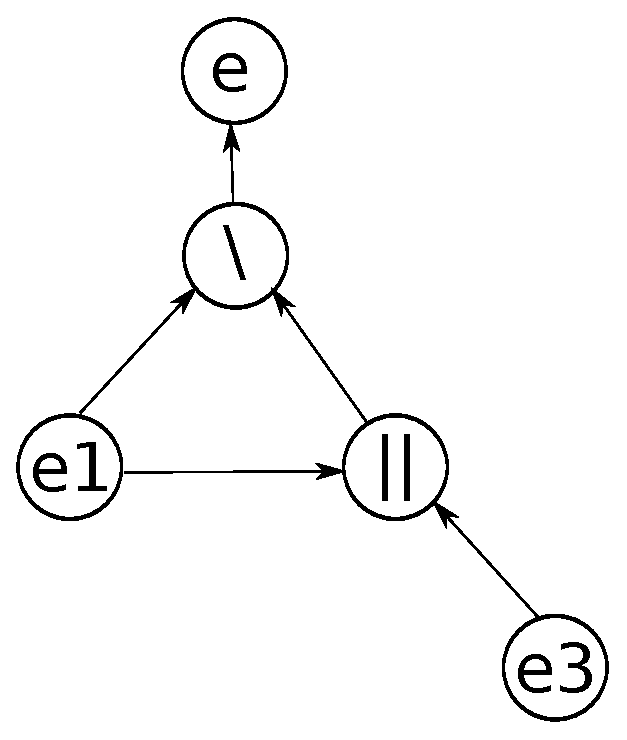
\includegraphics[width=0.3\textwidth]{graphics/event_node_except2_push}
  \label{failing_push_based_event_graph}
}
\subfigure[Push/Pull basierter Event-Graph] {
  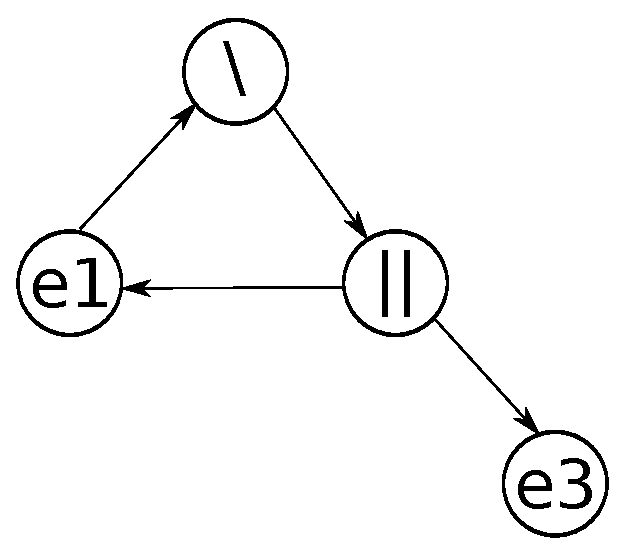
\includegraphics[width=0.3\textwidth]{graphics/event_node_except2_pull}
  \label{working_pull_based_event_graph}
}
\caption{Event-Graphen f"ur das Beispiel 2}
\end{figure}



\section{Beispiele}

Das Ziel dieses Abschnittes ist es, dem Benutzer die Verwendung von
Intervall-Events näherzubringen. Dazu wird gezeigt, an welchen Stellen sich
Intervall-Events sinnvoll einsetzen lassen. Bis auf das letzte Beispiel
existieren für alle Beispiele zwei Implementierungen. Eine Implementierung die
Intervall-Events verwendet und eine Implementierung die keine Events
verwendet.

\subsection{Implementierung eines Zustandsautomaten}
Zwei Beispiele zeigen die Verwendung von Intervall-Events bei der
Implementierung von Zustandsautomaten. Zustandsautomaten k"onnen hervoragend
durch die Verwendung von IntervallEvents implementiert werden, da
Zustandsautomaten immer vom Zustand abh"anige Reaktionen auf Events zeigen.

Zur Implementierung kann jeder Zustand des Automaten als ein Intervall
abgebildet werden. Alle in einen Zustand eingehende Transitionen werden dabei
als Start-Events des Intervalls verwendet und alle vom Zustand ausgehende
Transitionen werden als End-Event des Intervalls verwendet. Alternativ könnte
man auch die \after{}-Events des vorherigen Zustandsintervalls als Startevent
des nächsten Zustandes verwenden.

Durch diese Vorgehensweise ergibt sich eine bessere Wartbarkeit des
Quellcodes, da das Programmverhalten nicht mehr imperativ durch If-Statements
oder das Statemachine-Pattern beschrieben wird. Viel mehr wird das
Programmverhalten deklarativ durch Intevall-Events spezifiziert.

Im Rahme dieser Arbeit wurden zwei Zustandsautomaten implementiert. Der erste
Zustandsautomat besteht aus zwei Zuständen und soll dem Benutzer die
Vorgehensweise zur Implementierung eines Zustandsautomaten an einem stark
vereinfachten Beispiel zeigen. Der resultierende Zustandsautomat ist in Abb.
\ref{filetransfer_behaviour} zu sehen.

%\usepackage{graphics} is needed for \includegraphics
\begin{figure}[htp]
\begin{center}
  \includegraphics[width=0.15\textwidth]{graphics/tcp_stm.dot.eps}
  \caption{Verhalten einer Filetransfer-Verbindung}
  \label{filetransfer_behaviour}
\end{center}
\end{figure}


Im SimpleWebshop-Beispiel wird eine weitere Herangehensweise an die
Implementierung eines Zustandsautomaten mit Intervall-Events gezeigt. Häufig
lässt sich die Anzahl der benötigten Zustände und Transitionen durch die
Verwendung von paralellen oder hierarchischen Zustandsautomaten reduzieren.
Damit wird das Modell leichter verständlich aber die Implementierung des Modells
erschwert. 
Besonders die Implementierung von paralellen Zustandsautomaten ist zumeist sehr
unpraktisch. Der Zugriff auf den aktuellen Zustand der paralellen
Zustandsautomaten und das Verteilen von Events bereitet nämlich meist
Probleme. Daher werden oft zur Implementierung die Produktautomaten gebildet um
die paralellen Zustände aus dem Modell zu entfernen.

Dies ist bei der Verwendung von Intervall-Events zur Impelmentierung eines
Zustandsautomaten allerdings nicht zwingend notwendig. Die direkte
Implementierung eines paralellen Zustandsautomaten ist ohne Probleme möglich.
Die Verteilung der Events zum Ändern der Zustände und der Zugriff auf
benachbarte Zustandsautomaten ist einfach. 

Die Implementierung eines solchen Zustandsautomaten wie in Abb.
\ref{webshop_behaviour} dargestellt findet sich im Beispiel
interval\_simplewebhop.

%\usepackage{graphics} is needed for \includegraphics
\begin{figure}[htp]
\begin{center}
  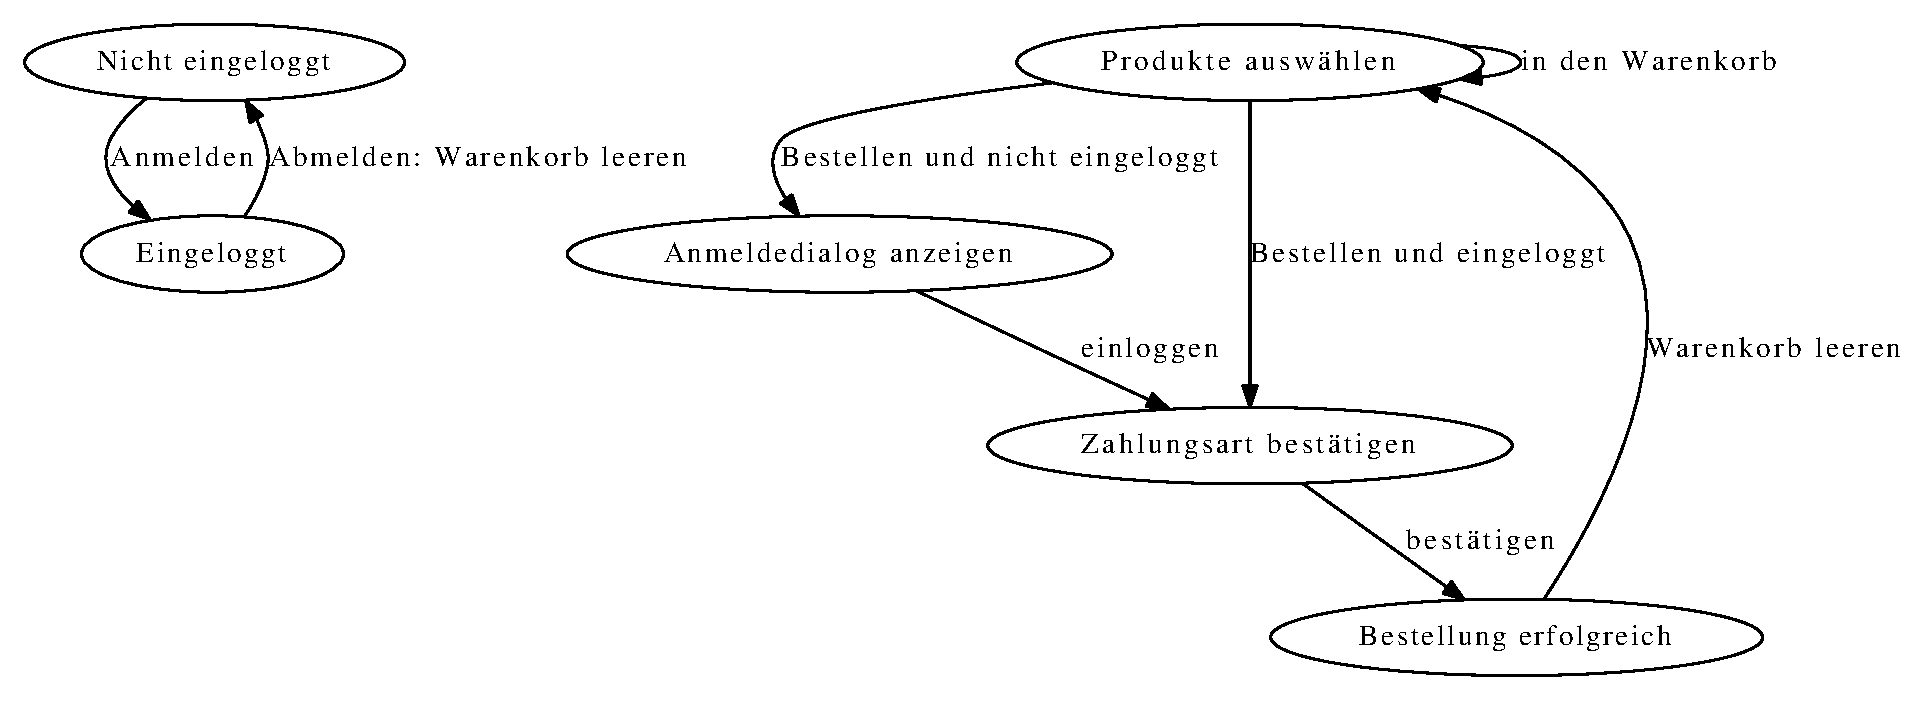
\includegraphics[width=0.6\textwidth]{graphics/webshop.dot.eps}
  \caption{Bestellvorgang in einem Web-Shop}
  \label{webshop_behaviour}
\end{center}
\end{figure}

\subsection{Implementierung einer FileTransfer-Komponente}
In viele Fällen wird ein Softwareentwickler keinen Zustandsautomaten
spezifizieren bevor die Software-Entwicklung beginnt. Viele zu lösende Probleme
lassen sich nämlich durch zwei oder drei Zustände beschreiben, sodass der
Entwickler nicht erst auf die Idee kommt, eine Zustandsmaschine zu
implementieren. Daher stellt sich die Frage, ob Intervall-Events auch in der
Praxis relevant sich um dem Entwickler beim Lösen von alltäglichen Problemen zu
helfen. Das nächste Beispiel zeigt daher die praktische Verwendung von
Intervall-Events:

Mit File-Sharing-Programmen können Benutzer über ein Computernetzwerk
Dateien austauschen. Wenn ein Benutzer eine Dateiübertragung anfordert, dann
fordert das File-Sharing-Programm von unterschiedlichen Hosts Teile der Datei
an. Die Hosts anworten dann mit den angeforderten Dateiteilen. Daher existiert
in den meisten File-Sharing-Programmen eine Komponente zum Steuern der
Dateiübertragungen. Diese Komponente verwaltet die bereits empfangenen
Dateiteile und kümmert sich darum, noch fehlende Tokens nachzufordern.

Bei der Implementierung einer solchen Komponente bietet sich die Verwendung von
Intervall-Events an. Das Verhalten der FileTransfer-Komponente kann fast
vollständig deklarativ erfolgen. 

\subsection{Implementierung von Ping-Pong}
Als größeres Beispiel wurde im Rahmen des Praktikums das Spiel
Ping-Pong implementiert. In diesem Spiel gibt es ein abgegrenztes Spielfeld mit
Wänden. Im Spielfeld befindet sich ein Ball der sich bewegt. Am Spiel teil
nehmen zwei Spieler die jeweils einen eindimensional beweglichen Schläger haben.
Der Schläger befindet sich vor dem Tor des Spielers. Ziel des Spiels ist es, den
Ball nicht in das eigene Tor zu lassen. Als kleine Erweiterung erscheinen auf
der Spielfläche Geschenke die das Spielverhalten abändern. Die Spielfläche des
Spiels ist in Abb. \ref{ping_pong} zu sehen.

\begin{figure}[htp]
\begin{center}
  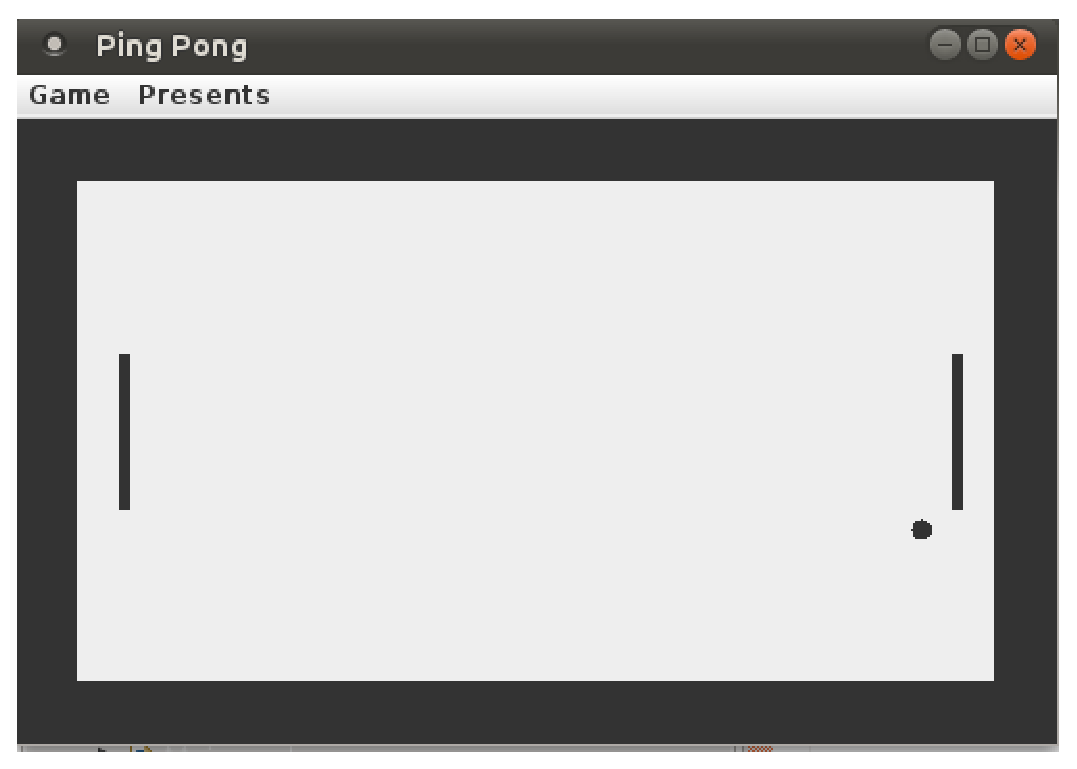
\includegraphics[width=0.6\textwidth]{graphics/pingpong.eps}
  \caption{Ping-Pong}
  \label{ping_pong}
\end{center}
\end{figure}

Das Spielmodell beinhaltet die Wände, den Ball, die Schläger, die Tore und
eventuell Geschenke. Jedes Objekt auf dem Spielfeld hat eine Position und eine
Geschwindigkeit. Allerdings wurde bei der Implementierung des Spiels von der
Klassischen Herangehensweise abgewichen. Klassischerweise besteht ein Spiel aus
einer Spielschleife in der die folgenden Aktionen immer wieder ausgeführt
werden:
\begin{itemize}
  \item Abfragen der Benutzereingaben
  \item Berechnung der Änderungen im Spiel-Modell. Also die Positionsänderung
  des Balls und der Schläger.
  \item Rendern des Spielmodells zu einer Grafik
  \item Warten bis die nächste Iteration notwendig wird. Ohne diese Wartezeit
  hätte man möglicherweise eine zu hohe Frame-Rate.
\end{itemize}

Diese Ansatz ist allerdings nicht Event-Orientiert und wurde daher im Beispiel
nicht verwendet. Stattdesen wird im Beispiel ein Timer verwendet, der alle 50ms
eine Positionsänderung der Objekte und und das Neuzeichnen der Spielfläche auslöst.
Solange ein Spieler eine Bewegen-Taste drückt ist ein Intervall-Event aktiv das
die Geschwindigkeit des Schlägers ändert\footnote{Dies ist übrigens ein
eleganter Workaround für einen Bug in der Java AWT. Mehr Informationen zum
diesem Fehler finden sich unter
bugs.sun.com/view\_bug.do?bug \_id=4153069}.

Weiterhin werden Intervall-Events eingesetzt, um das Zeitmodell des Spiels
abzubilden. Geschenke beispielsweise sollen nur für eine definierte Zeit
vorhanden sein. Diese Funktion wurde durch ein Intervall-Event realisiert, das
vom Beginn der Sichtbarkeit für eine gewisse Zeit aktiv ist. 

\subsection{Zusammenfassung}
Fasst man die Beispiele zu einem Fazit zusammen, so lässt sich sagen, dass durch
die Verwendung von Intervall-Events ein deklaratives Implementieren von
zustandsbasierten Problemen möglich ist. Dies verbessert die Lesbarkeit und die
Wartbarkeit des Quellcodes. Allerdings gibt müssen zwei Schwierigkeiten bei der
Verwendung von Intervall-Events bedacht werden: Zum einen ist Vorsicht bei der
Verwendung von rekursiven Definitionen geboten. Eine Verwendung dieser
Konstrukte erfordert das Markieren des Start-Intervalls mit \textit{lazy} und
die Definition eines Startevents um eine korrekte Initialisierung der rekursiven
Definition vorzunehmen.

Zum anderen ist es wichtig, ein exaktes Event-Modell für eingehende und
ausgehende Events zu erstellen. Es ist wichtig, zwischen Events die Transitionen
auslösen können und Events die Aktionen zur Folge haben zu trennen. Ist diese
Trennung nicht exakt genug, dann könnten eventuell Aktionen ausgeführt werden,
die im akutellen Intervall nicht zulässig sind. 

Beachtet man diese Entwurfskriteren, so ist es durch Intervall-Events möglich,
auf einem hohe Abstraktionsnivea Software zu entwicklen. 


\section{Resümee}
Durch die Verwendung von Intervall-Events kann man zustandsbasierte
Probleme deklarativ lösen. Man spart sich dann die imperative Implementierung
eines Zustandsautomaten. Dies verbessert die Verständlichkeit des Quellcodes und
verringert somit die Wartungskosten für ein Software-Projekt. 

Allerdings bringt die Verwendung von Intervall-Events auch Probleme mit sich.
Die Deregistrierung von Events obliegt nämlich dem Benutzer. Wenn ein Benutzer
nicht länger benötigte Events nicht wieder vom Event-Graph abkoppelt, dann
können die zu den Events gehörenden Objekte nicht freigegeben werden. Dies hat
zur Folge, dass der Speicherverbrauch der Anwendung möglicherweise immer weiter
ansteigt. 

Die Intervall-Events können nicht automatisch deregistriert werden, da nicht
bekannt ist, ob der Benutzer noch Interesse am Intervall-Event hat. Es könnte
sein, dass ein Intervall-Event nur ein einziges mal für den Benutzer von
Interesse ist. Möglicherweise benötigt der Benutzer das Intervall-Event aber
mehrfach. Wichtig ist daher, dem Benutzer die Deregistrierung der Events
nahezulegen.

\section{Ausblick}
Der nachfolgende Ausblick betrifft Events im Allgemeinen und Intervall-Events im
speziellen.

Zukünftig sollte sich die Intervall-Events-Library in zwei Richtungen
weiterentwickeln. Zum einen ist es wichtig den Benutzer bei der Deregistrierung
von nicht mehr benötigten Intervall-Events zu unterstützen. Und zum anderen kann
die Intervall-Events-Library ihr volles Potential nur ausspielen, wenn
die Implementierung effizient in Multithreading-Szenarien funktioniert.

\subsection{Konzepte zur Vereinfachung der Deregistrierung von Reactions}

Möglicherweise könnte man eine Datenfluss-Analyse im Kontrollfluss-Graph
vornehmen, um nach Events zu suchen. Wenn ein Event gefunden wurde, auf den eine Reaction
registriert wurden, muss sichergestellt werden, dass auch eine Reaction wieder
entfernt wird. Allerdings ist das ein "`Best-Efford"'-Ansatz. Man kann auf diese
Weise nicht in allen Fällen sicherstellen, dass die verwendeten Events immer
korrekt aufgeräumt werden.

Außerdem könnte man dem Benutzer Zugriff auf den Funktionszeiger von
anonymen Funktionen bereitstllen. Wenn Intervall-Events in Methoden verwendet
werden, sind diese Intevalle dann meist nur selten aktiv und müssen nach 
zeitlich kurzer Zeit wieder deregistriert werden. Allerdings sollten dabei 
keine anonymen Funktionen verwendet werden. Anonyme Funktionen können nämlich 
nicht deregistriert werden, da keine Möglichkeit besteht, an den Funktionszeiger
der anonymen Funktion zu kommen, um diese wieder zu deregistrieren.

\subsection{Effiziente und skalierbare Funktionsweise in
Multithreading-Szenarien}
Die Threadsicherheit ist eine überaus wünschenswerte Eigenschaft für
Intervall-Events. In der Zukunft werden Interaktionen zwischen verschiedenen 
Thread zunehmend immer wichtiger. Das Konzept der Events und der
Intervall-Events ist natürlich nicht auf sequenzielle Prozesse beschränkt und
skaliert sehr gut auch auf Thread- und Prozess-Ebene. Diese Tatsache
manifestiert sich in der Existenz von Messageoriented
Middleware. 

Um die Intervall-Events-Implementierung Multithreading-sicher zu machen, muss
geprüft werden, ob alle Zustandsänderungen des Aktiv-Zustands eines
Intervall-Events multithreading-sicher sind. Weiterhin muss die Events-Library
Multithreading-sicher sein.

\listoffigures\addcontentsline{toc}{section}{\listfigurename}
\end{document}
